\chapter{恒星大气}
\paragraph{光强和辐射流量关系}
\begin{equation}
  F=\int I \cos\theta d\Omega=\int d\phi\int I \cos\theta\sin\theta d\theta =\sigma T^4
\end{equation}

\paragraph{能量密度}
\begin{equation}
  u={1\over c}\int I d\Omega=aT^4
\end{equation}

\paragraph{辐射压}
\begin{equation}
  P_\mathrm{rad}={2F \cos{\theta}\over c}={1\over3}aT^4={1\over 3}u
\end{equation}

\section{恒星不透明度}
前文提到恒星并不是理想黑体,产生的光谱也就不是严格的黑体谱,我们所观测到的恒星光谱主要来自恒星的光球层,但是恒星大气中存在的各种金属(天文中指比氢、氦重的元素)也会产生相应的谱线(参见\ref{kirchhoffs}节基尔霍夫定律)。

对于恒星的温度,我们也有多种定义:
\begin{itemize}
  \item 有效温度,通过斯特藩-玻尔兹曼定律(\ref{eq:stefan}),即发光能力来定义
  \item 激发温度,通过玻尔兹曼方程(\ref{eq:boltzmann}),即原子能级分布来定义
  \item 电离温度,通过萨哈方程(\ref{eq:saha}),即原子电离情况来定义
  \item 动力学温度,通过麦克斯韦-玻尔兹曼分布(\ref{eq:maxwell}),即粒子速率分布来定义
  \item 色温度,通过普朗克公式(\ref{eq:planck}),即恒星连续谱与黑体谱拟合来定义
\end{itemize}

其中有效温度是我们最常使用的,而其他温度只在恒星中的一些特殊区域应用,尽管这些温度定义不同,但是对于一团处于\textbf{热力学平衡}的理想气体,它们都是相同的。

\paragraph{热力学平衡}
不受外界作用的条件下,系统能够长久保持而不会发生变化的一种热力学状态,即内部能量产生与释放速率相等


然而,恒星并不是完全处于热力学平衡,不同位置的温度并不相同。但是如果处于\textbf{局部热力学平衡},即在粒子或光子的\textbf{平均自由程}(自由运动不与其他粒子发生相互作用的平均距离)内,温度变化很小,我们可以认为该区域处于相同温度。

对于光子来说,其平均自由程为:
\begin{equation}
  \ell={1\over \kappa_\lambda \rho}={1\over n \sigma_\lambda}
\end{equation}

其中$\kappa_\lambda$和$\sigma_\lambda$分别是不透明度(吸收系数)和散射截面,大小都与波长相关。

由于不能单纯地依靠光通过的距离来评估其衰减程度,因为相同距离,不同介质对光有不同的吸收效果,因此定义\textbf{光深$\tau_\lambda$来描述光子在传播过程中的平均碰撞次数}:
\begin{equation}
  \tau_\lambda=\int^s_0{ds\over \ell}=\int_0^s\kappa_\lambda\rho\,ds
\end{equation}

对于一定尺度的介质,$\tau\gg1$为光厚介质,$\tau\ll1$为光薄介质。

\paragraph{不透明度的来源}
\begin{itemize}
  \item 束缚-束缚跃迁(bound-bound transitions),光子如果能量与原子能级差吻合,会被电子吸收,跃迁到高能级
  \item 束缚-自由吸收(bound-free absorption),光子能量足够大时,能够直接电离电子,使电子进入自由态,此为光致电离。典型的例子是\textbf{巴尔末跳变},由于电子最终被电离,因此吸收光子的频率不像束缚-束缚跃迁要满足能级差,第一激发态的电子会对大于电离能(波长小于364.6\;nm)的光子全吸收,该区域谱线强度整体下降,如图\ref{fig:balmerjump}。
  \item 自由-自由吸收(free-free absorption),在离子附近的自由电子可以吸收光子,从能量较低的自由态进入能量更高的自由态,这是轫致辐射的逆过程
  \item 电子散射,与自由电子发生汤姆孙散射
\end{itemize}

\begin{figure}[hbt]
  \centering
  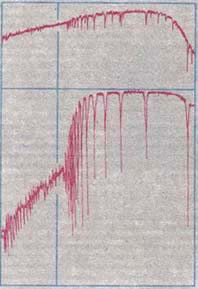
\includegraphics[width=4cm]{chapters/09/balmerjump}
  \caption{巴尔末跳变。图中蓝线对应波长364.6\;nm,氢的巴尔末线系的波长}
  \label{fig:balmerjump}
\end{figure}

由于不透明度和波长与介质有关,为了研究简便,我们通常会使用\textbf{罗斯兰平均不透明度}来替代,即对全波段的不透明度做加权平均,使其只对介质本身依赖
\begin{equation}
  {1\over \bar\kappa} \equiv{\displaystyle\int_0^\infty {1\over \kappa_\upsilon}{\partial B_\upsilon(T)\over \partial T}\,d\upsilon \over \displaystyle\int_0^\infty{\partial B_\upsilon(T)\over \partial T}\,d\upsilon}
\end{equation}

\section{辐射转移}
\subsection{光子辐射过程}
电子吸收光子会跃迁到高能级,但在高能级并不稳定,一段时间之后还会再落回低能态,这会伴随着辐射光子,因此光在经过介质时,\textbf{介质既会吸收光子也会辐射光子}。因此定义了发射系数$j_\lambda$,并用\textbf{辐射转移方程}来描述光强变化:
\begin{equation}
  {dI_\lambda \over d\tau_\lambda}=S_\lambda-I_\lambda
\end{equation}

其中$S_\lambda={j_\lambda\over \alpha_\lambda}$为原函数,若为常数,可得到方程特解:
\begin{equation}
  I_\lambda(\tau_\lambda)=\underbrace{I_{\lambda,0}e^{-\tau_\lambda}}_\text{入射光本身的衰减}+\underbrace{S_\lambda(1-e^{-\tau_\lambda})}_\text{介质对光强的净效果(吸收和辐射)}
\end{equation}

在局部热平衡的情况下,原函数$S_\upsilon=B_\upsilon$,即黑体辐射。

如果假设光子的传播方向时随机的,散射方向也是随机的,那么可以认为光子传播过程是\textbf{随机游走}过程,如果光子不被吸收,只被散射,它要穿过厚度为$d$的介质会被散射$N=d^2/\ell^2$次。

\paragraph{爱丁顿近似下的温度垂直分布}
\begin{equation}
  T^4={3\over 4}T_e^4\left(\tau_\upsilon+{2\over3}\right)
\end{equation}

其中$T_e$为有效温度,可以发现当$\tau_\upsilon=2/3$时,$T=T_e$,也就是说我们能看到的最深的光是来自恒星表面以下2/3光深处(表面$\tau_\upsilon=0$)。

\subsection{光谱线轮廓}
如果光子被吸收,就会恒星的连续谱中产生如图\ref{fig:spectrum}的谱线,被吸收的越多,则产生的``凹陷''越深,谱线越强,因此为了定量衡量谱线强度,定义\textbf{等值宽度}:
\begin{equation}
  W=\int{\displaystyle F_c-F_\lambda \over \displaystyle F_c}\,d\lambda
\end{equation}

即如图\ref{fig:spectrum}中定义一个矩形,高度和边缘相同,面积和``凹陷''面积相同,对应宽度即为等值宽度。

\begin{figure}[hbt]
  \centering
  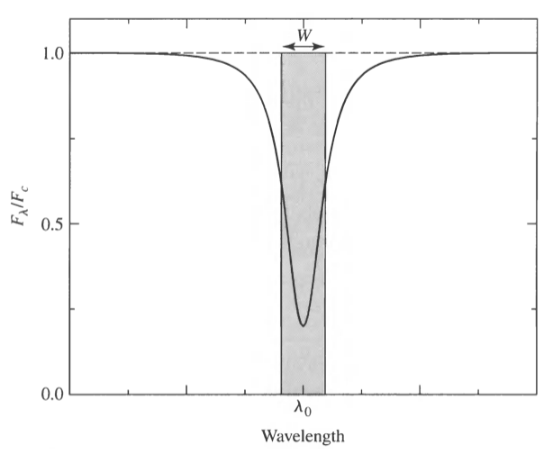
\includegraphics[width=10cm]{chapters/09/spectrum}
  \caption{典型的光谱线轮廓}
  \label{fig:spectrum}
\end{figure}

\subsection{谱线增宽机制}
前面讲过(\ref{kirchhoffs}节),电子能级跃迁才会在产生谱线,且谱线频率与跃迁的能级差相对应,那么谱线应该是一根严格的线,但是实际中会有几个主要机制会使谱线增宽:
\begin{itemize}
  \item \textbf{自然增宽},由于海森堡不确定性原理(\ref{uncertainty}节),原子在激发态上只能存在短暂瞬间,即在某能级的时间间隔$\Delta t$很小,因此对应的能级就无法精确测量,存在的误差$\Delta E\approx\hbar/\Delta t$就会较大,也就导致激发出的光子频率不是精确值,从而谱线产生增宽。
  \item \textbf{多普勒增宽},由于原子处于热运动,在发射光子时会产生多普勒频移,从而增宽
  \item \textbf{碰撞增宽(压强增宽)},碰撞会使激发态电子的寿命发生变化,本质与自然增宽相似
\end{itemize}